%
% File naaclhlt2016.tex
%

\documentclass[11pt,letterpaper]{article}
\usepackage{naaclhlt2016}
\usepackage{times}
\usepackage{latexsym}
\usepackage{graphicx}
\usepackage[]{algorithm2e}

\naaclfinalcopy % Uncomment this line for the final submission
\def\naaclpaperid{***} %  Enter the naacl Paper ID here

% To expand the titlebox for more authors, uncomment
% below and set accordingly.
\addtolength\titlebox{-1in}    

\newcommand\BibTeX{B{\sc ib}\TeX}


\title{EECS 595 - Semi-Supervised learning of Patterns in Text using Sequence Learning}

% Author information can be set in various styles:
% For several authors from the same institution:
% \author{Author 1 \and ... \and Author n \\
%         Address line \\ ... \\ Address line}
% if the names do not fit well on one line use
%         Author 1 \\ {\bf Author 2} \\ ... \\ {\bf Author n} \\
% For authors from different institutions:
% \author{Author 1 \\ Address line \\  ... \\ Address line
%         \And  ... \And
%         Author n \\ Address line \\ ... \\ Address line}
% To start a seperate ``row'' of authors use \AND, as in
% \author{Author 1 \\ Address line \\  ... \\ Address line
%         \AND
%         Author 2 \\ Address line \\ ... \\ Address line \And
%         Author 3 \\ Address line \\ ... \\ Address line}
% If the title and author information does not fit in the area allocated,
% place \setlength\titlebox{<new height>} right after
% at the top, where <new height> can be something larger than 2.25in
\author{Cyrus Nikolaidis, Hrishikesh Rao, Aravind Bharathy,\and Graham Palmer}
 

\date{}

\begin{document}

\maketitle

\begin{abstract}
 Classifying text samples is a classic problem in Natural Language Processing, and there is a wide variety of available methods to perform such a task given a labeled dataset. The goal of this project is to attempt to apply these methods in a semi-supervised way - that is, with two sets of samples, one labeled, one unlabeled, as training data, in such a way that the resulting model has better performance than if it were trained on just labeled data. In doing this, we use LSTM/GRU, powerful models for sequence learning that can be applied to language modeling.
\end{abstract}

\section{Introduction}

Several of the topics studied in this course relate to creating models of language - which models a "language" as a probability distribution of possible strings.

We can create these models of language using labeled samples of text, and thus determine the "language" (or, more generally, classification) of an unlabeled sample of text with high accuracy. An example is using a unigram model to guess whether a piece of text is a sentence in English or French, or to predict the sentiment of a piece of text.

An issue with this is that many of these labelings are tedious to create. The goal of this project is to create a classifier that, using a labeled dataset and a unlabeled dataset, can create a classifier of higher quality than what we could create given only the labeled dataset.

This initially seems impossible - what meaningful information do the text samples carry without labels? However, our intuition that this is possible to do is motivated by observing other unsupervised training methods, such as k-means. In this method, cluster centers for a set of points are found through repeated iteration of 1) assigning each point a cluster center, and 2) choosing new cluster centers based on the points belonging to each cluster. 

The reason this works is because points in the same cluster have similar features, and the model can recognize this even when the points are not labeled. One can imagine that one can use a language model, which outputs a probability ("a distance") for each class label can be imagined as a cluster center for a set of text samples, and we can repeatedly retrain the language models and label unlabeled text data to achieve a similar result as with the k-means algorithm (indeed, both of these methods would function as a special case of the E-M unsupervised learning algorithm). We could improve this by using a semi-supervised method to initialize the language model using correct data to set it on the "right path" and then use the unsupervised methods to leverage the rest of the data.

As it turns out, there are many ways of applying unsupervised learning methods to text classifications. We will explore an option we find effective in this project.


\section{Related Work}

There has been extensive work in both the areas of semi-supervised training language models and the use of sequence models like LSTMs and GRUs for text classification, although it is not immediately obvious that anyone had published anything about using these two methods in conjunction, as we intend to do here. Our application of both topics here draws heavily from past work on the topics. 

\cite{Sundermeyer:12} is an example of a recent work which explores the use of LSTM neural network in language modeling. Since the time of it's publication, LSTM has become a commonly used model for the original supervised version of this task, so our use of it here is not at all unprecedented, and the exact model architecture can be drawn from these past uses.

\cite{Nigam:12} and \cite{mihalcea2004co} explore different methods (E-M algorithm, self-training, and co-training) for solving language problems in a semi-supervised way. The way we are currently planning to execute the semi-supervised learning process is via self-training, described in \cite{mihalcea2004co}.

Finally, there has been other work in attempting to use "Deep Clustering" \cite{xie2016unsupervised} and even "Deep clustering for NLP". \cite{dai2015semi} Both of these conclude that unsupervised methods using neural nets can be effective.

\section{Methods}

\subsection{Sequence Learning Model Description}

\begin{figure}
	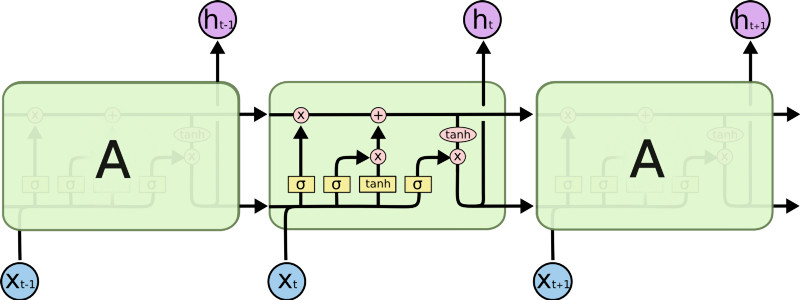
\includegraphics[scale = .25]{gru}
	\caption{An example of an LSTM cell, one possible recurrent component of the model used in this project \cite{lstm:15}}
\end{figure}

\begin{figure}
	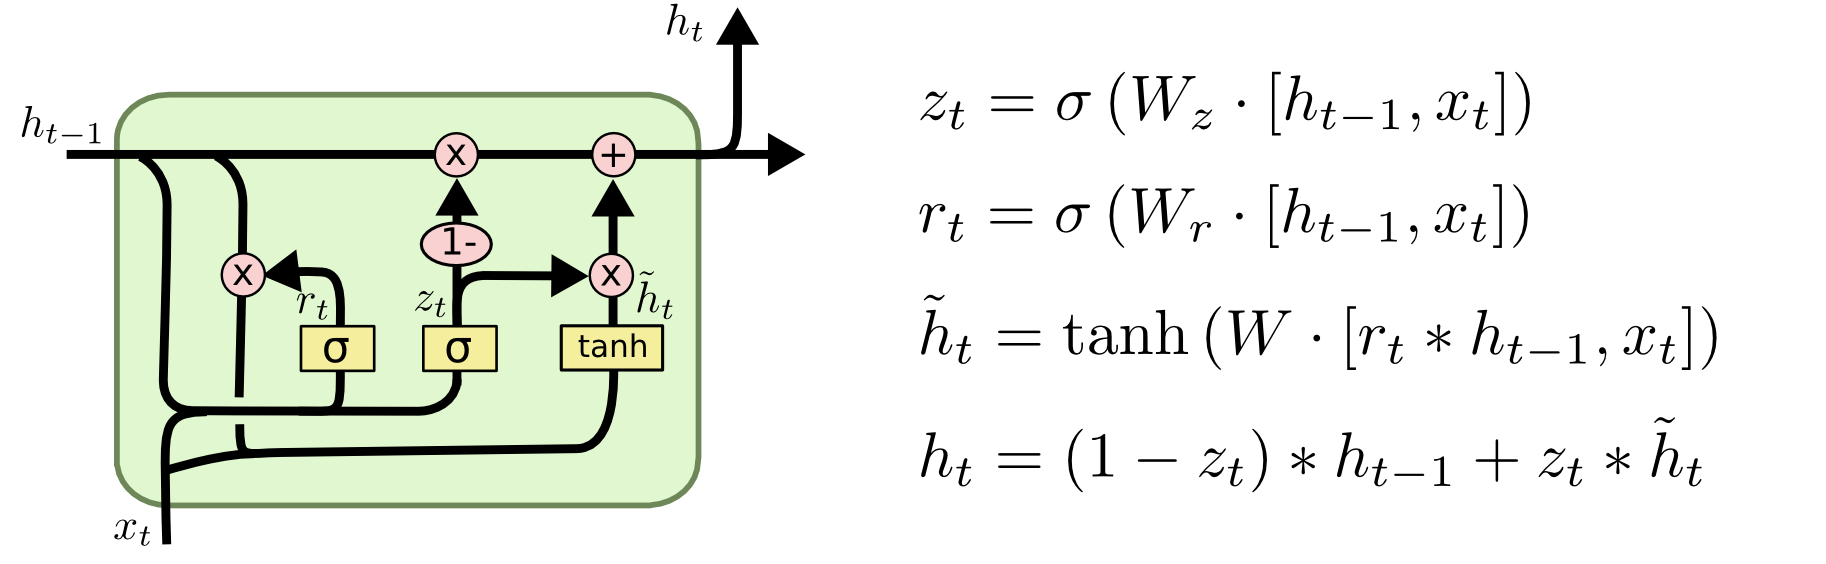
\includegraphics[scale = .35]{lstmcell}
	\caption{An example of an GRU cell, one possible recurrent component of the model used in this project \cite{lstm:15}}
\end{figure}

LSTMs \cite{hochreiter1997long} and GRUs are highly effective recurrent neural network structures, particularly useful in natural language contexts. \cite{Sundermeyer:12}  In this project we will treat these structures largely as a black box for a general "language model". That is, when trained on samples of text labeled as being in one of $n$ languages, we assume the model outputs for an input string $n$ values proportional to the probability that the string belongs to each of the languages. This can be thought of as simply a classifier.

The difference between LSTMs and GRUs is that GRUs can train on less data but are less capable of learning "long distance" dependencies within a sequence. \cite{lstm:15} In this project we asses which one of these models is useful for the classical supervised sentence classification and tasks and then  move to use that model for the unsupervised task.

\begin{figure}
	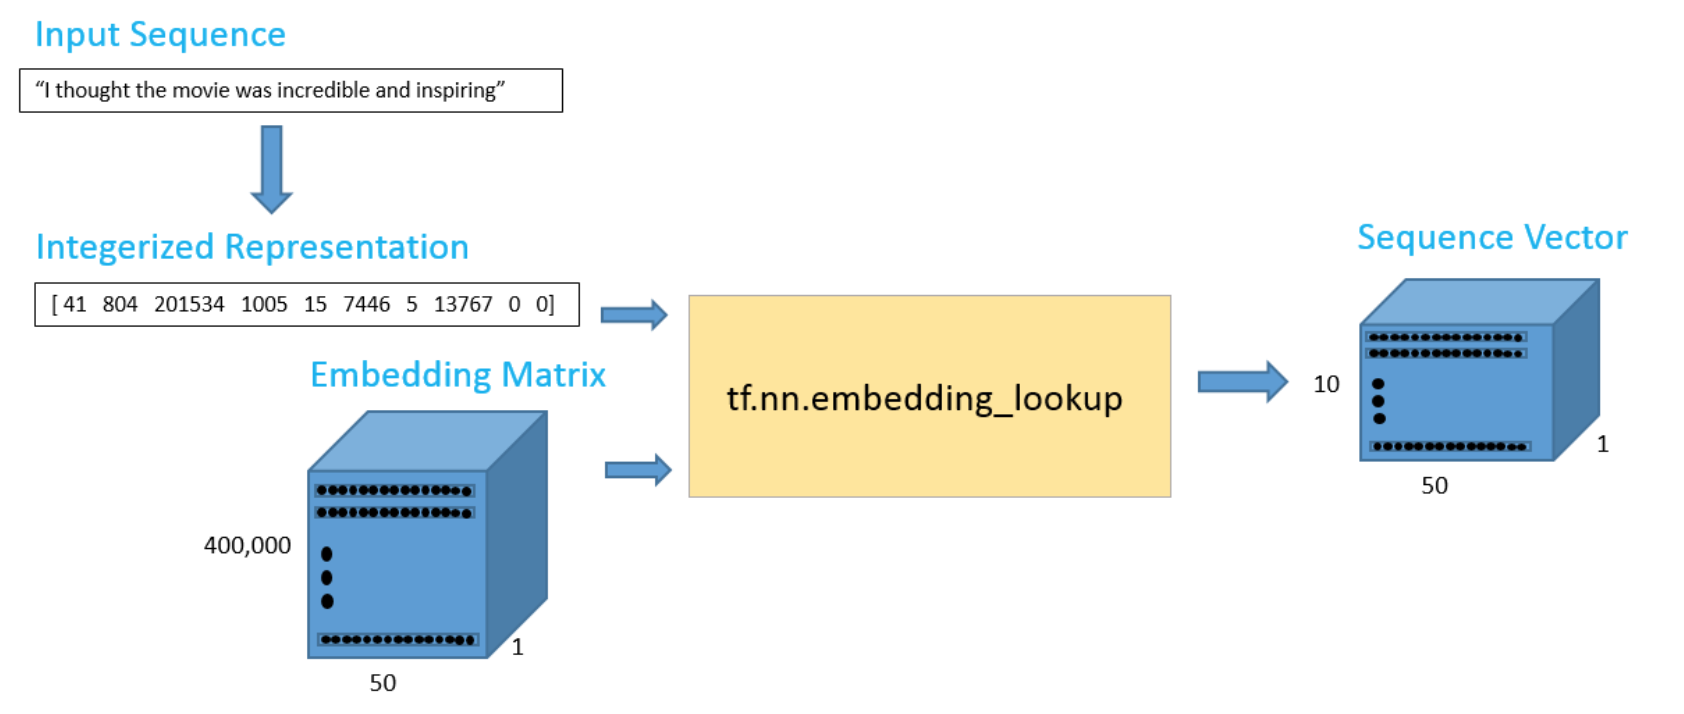
\includegraphics[scale = .23]{embeddings.png}
	\caption{Method of generating sequences using word embeddings.}
\end{figure}

\begin{figure}
	\includegraphics[scale = .27]{LSTM}
	\caption{Input and output of Sequence Learning model.}
\end{figure}

The method we use to generate sequence predictions (as a set of class label probabilites) with LSTM as follows:

\begin{itemize}
	\item In order to translate our word sequence data effectively into meaningful states, we use pretrained word embeddings. These word embeddings are created in an unsupervised manner to contain as much information about the word as possible while still remaining relatively low dimensional.
	\item We pass these sequences through an LSTM/GRU to retrieve an output state.
	\item We compute a set of class probabilities from this state by passing the output state through a linear and softmax layers in succession.
\end{itemize}

In order to train the model, we minimize a loss function, which is the cross-entropy of the predicted class probabilities and the ground truth labels:

\begin{equation}
	H_{y'} (y) := - \sum_{i} y_{i}' \log (y_i)
\end{equation}



\clearpage
\subsection{Semi-Supervised Learning Methods}

Now that we have a method for creating supervised models for text classification, we need to describe a way to effectively use unlabeled information.

The algorithm we are planning to use for unsupervised learning is called \textbf{self learning}, which is described in \cite{mihalcea2004co}, and works as follows:

\begin{algorithm}[H]
 \KwData{input sequences, input labels, unlabeled sequences}
 \KwResult{Model for predicting class labels }
 threshold := $\in [0, 1]$;
 
 training sequences := input sequences;
 
 training labels := input labels;
 
 i := 0;
 
 \While{i $<$ some number of iterations}{
  Train LSTM model on training sequences, training labels\;
  Predict label and confidence score for each sequence in unlabeled sequences\;
  \For{each unlabeled sequence}{
  	\If{confidence $>$ threshold}{
  		Add sequence, predicted label to training sequences\;
  	}
  } 
  
  i += 1;
 }
 \caption{Self Learning}
\end{algorithm}

In other words this algorithm repeatedly trains a classifier, predicts labels for unlabeled data, and then adds the predicted labels for data for which it is most confident about to the training data.

This method can be analogized to the K-Means algorithm often used in unsupervised learning, and in general can be said to be an instance of the E-M algorithm \cite{dempster1977maximum}. The parameters of the LSTM and linear layer can be thought of as "the cluster centers" and the predictions of the model can be thought of as the "cluster assignments".

Note that we also train on the small fraction of supervised labels while doing this. The goal of this is to hopefully "set the model parameters on the right path" towards converging on a correct solution.

\subsection{Choice of threshold}

A nontrivial aspect of our method above is the use of a confidence threshold. The confidence threshold exists so that the model only trains on unlabeled data that it believes it has likely classified accurately. For each prediction made by our model, a confidence score naturally exists (since the output is a probability the model assigns to each class). We want to choose a threshold that maximizes the accuracy of examples above that threshold (so that we give the model accurate information to train on) while also maximizing the number of examples meeting this threshold (so that the E-M process actually gains information with each iteration). We found that a threshold of $.99998$ allowed for a large amount of examples with relatively high predicted accuracy. Our assertion that this method could work here depends on the notion that a situation in which all examples were classified perfectly (and thus the models would classify the examples correctly) would most likely have the least loss, and we must hope that the model parameters converge to this minimum with each unsupervised iteration (something that is very probable in basic k-means but is not clearly as likely here).

\begin{figure}
	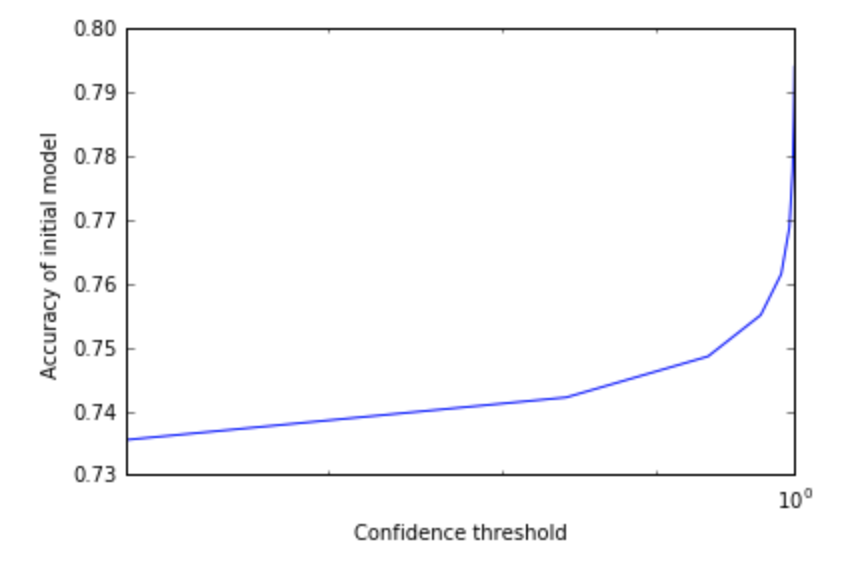
\includegraphics[scale = .45]{conf-acc}
	\caption{Confidence of the initial model vs. accuracy of predictions}
\end{figure}

\begin{figure}
	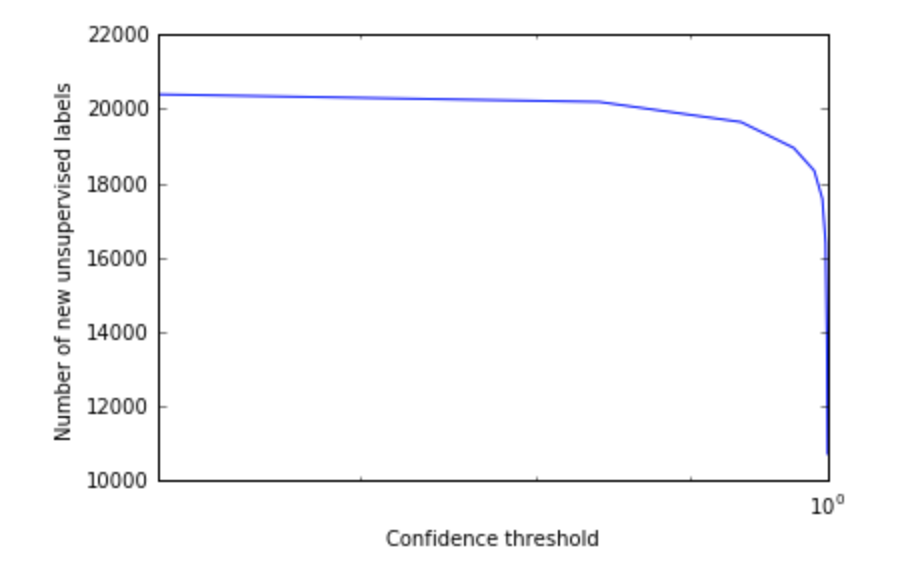
\includegraphics[scale = .45]{conf-num}
	\caption{Confidence of initial model vs. number of predictions with that confidence}
\end{figure}

\clearpage

\section{Experimental Setup}

\subsection{Text classification datasets}

The goal is to find datasets containing samples of text annotated with some small finite set of class labels. Due to the limitations of our model, it is necessary to find datasets which are sufficiently large (at least 10000 examples) and for which the differences between sentences are not so subtle that the supervised LSTM/GRU model cannot learn to distinguish between classes. 

The dataset we are currently leveraging is the \textbf{IMDB Movie Reviews dataset}, a dataset of 25000 examples of movie reviews labeled by sentiment (half positive and half negative). Given that users submit ratings along with the review texts, manual data annotation was not necessary here. We have observed that this works well with our original supervised LSTM method (81\% test set accuracy) and even better with the supervised GRU method (87\% test set accuracy) so should be fine to use for the semi-supervised process.

An example of a "positive sentiment" review in the dataset that the model learns to recognize: \begin{verbatim}
	This is a great movie. 
	It is based on a true story. 
	This movie helps not only children 
	cope with losses, 
	but older people as well. 
	Hope everyone will enjoy it!!!
\end{verbatim}

In addition to this dataset we are looking into experimenting with a number of other datasets (Newsgroup classifications, Music Genre classifications, etc.)

\subsection{Word embeddings}

We also obtain our word embeddings from an outside source. Specifically we use pretrained word embeddings by GloVe. \cite{pennington2014glove}  of dimension 50.

\begin{figure}
	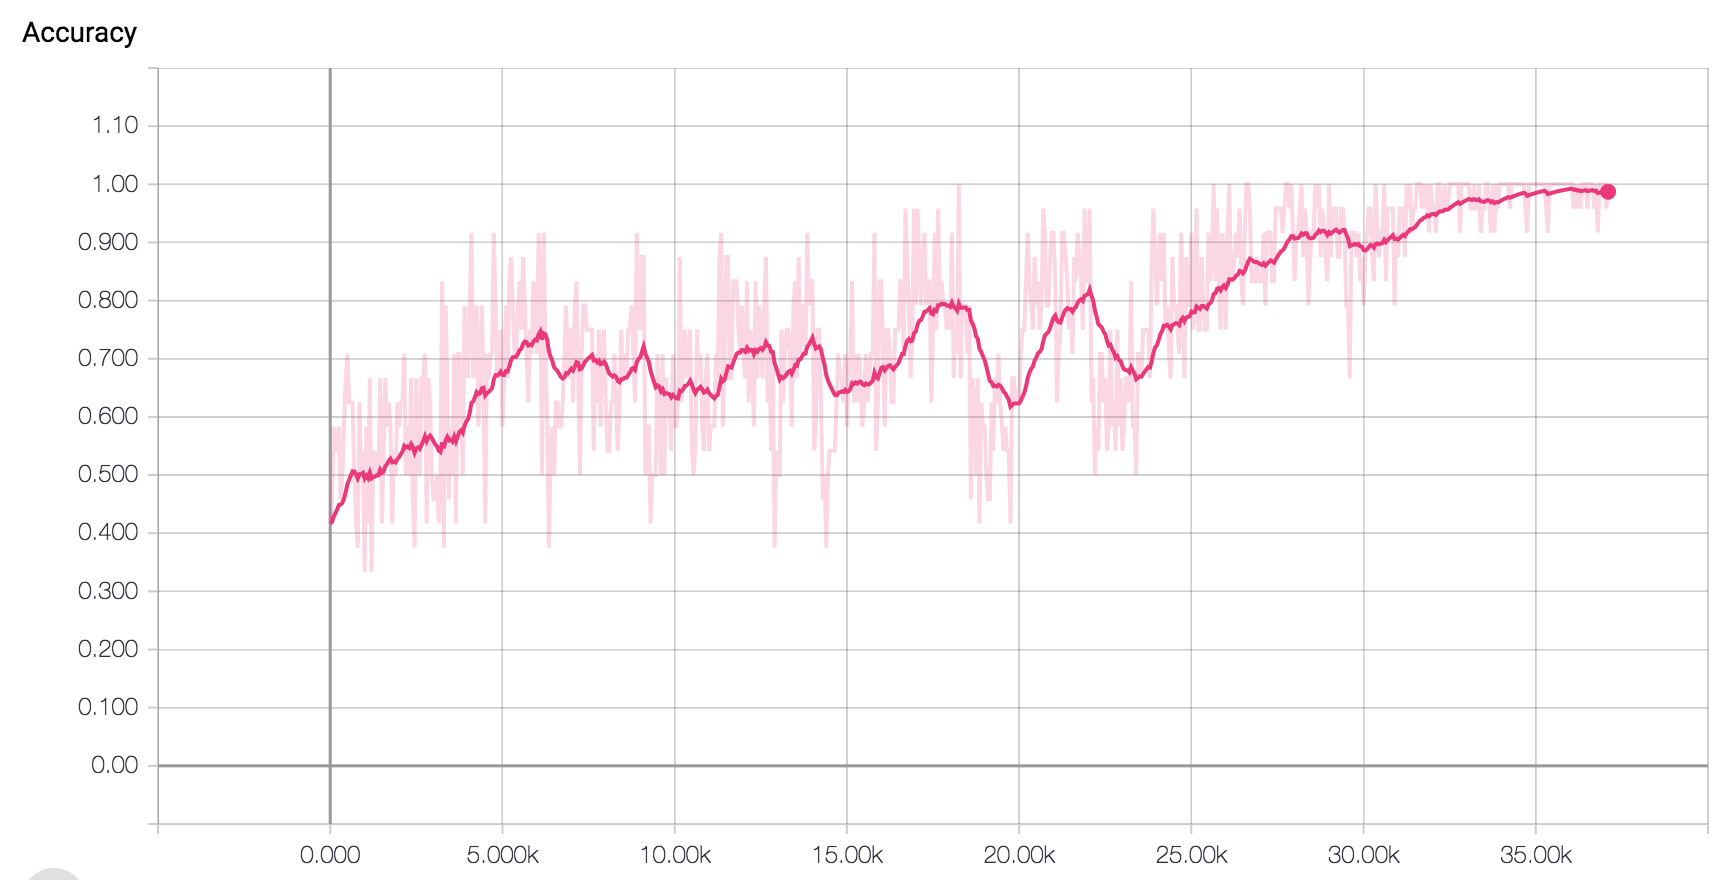
\includegraphics[scale = .27]{accuracy}
	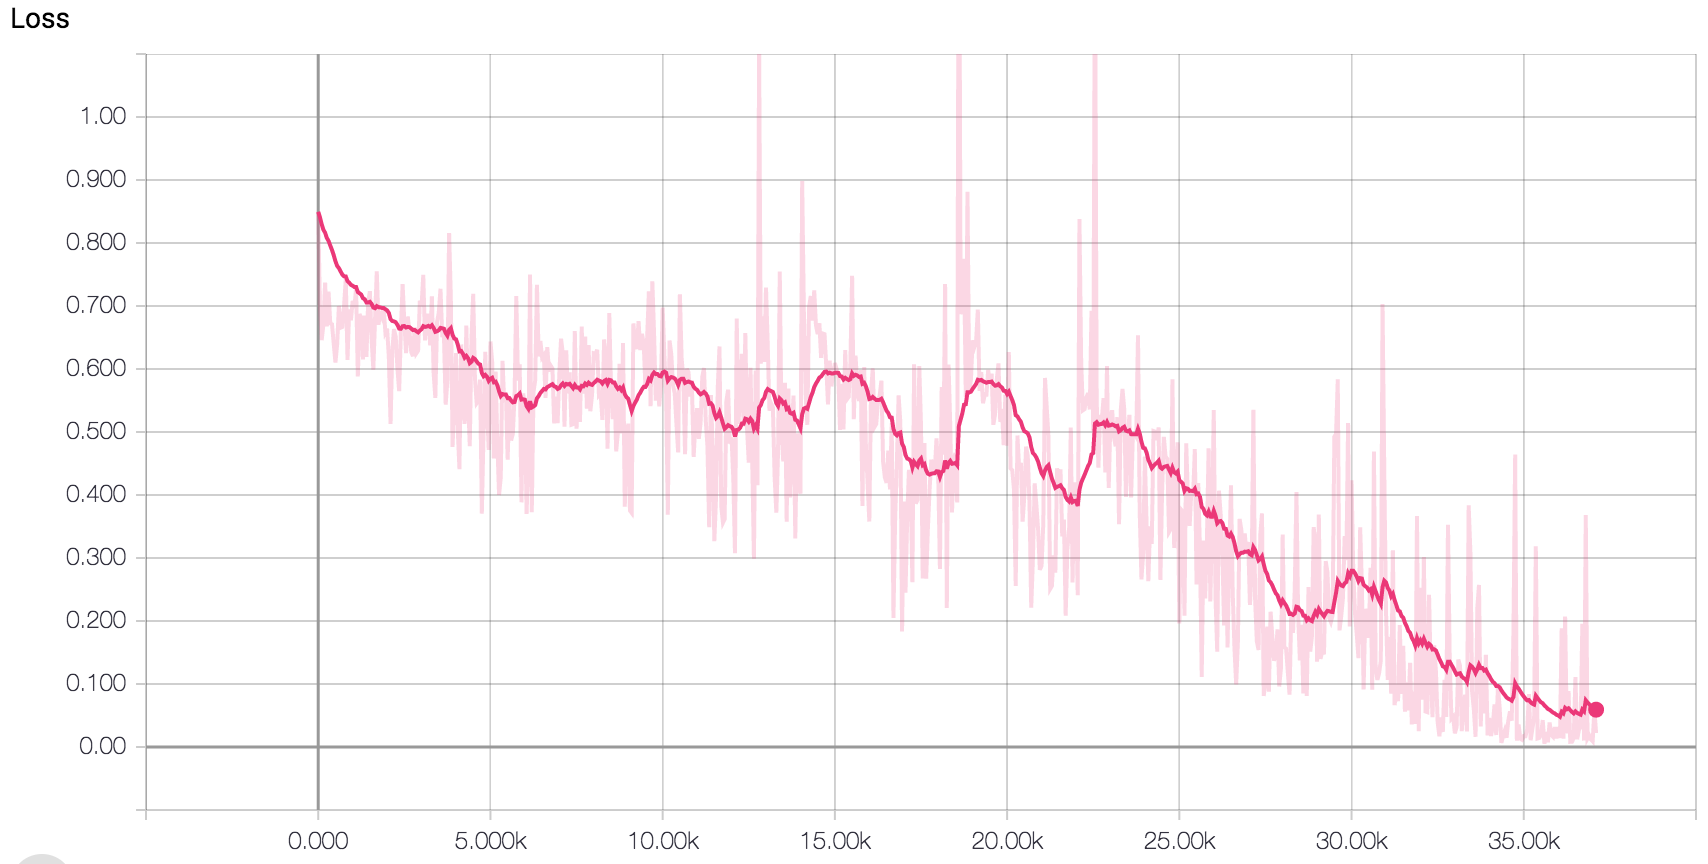
\includegraphics[scale = .27]{loss}
	\caption{Accuracy and loss of our initial supervised model when trained on supervised labels on the IMDB movie reviews dataset as a function of training iterations}
\end{figure}

\subsection{Evaluation metrics}

For any given dataset, by holding out a portion (we chose to make this proportion .1) of the data to be a test set, our models can be compared simply with the metric of classification accuracy, the proportion of the test set for which the model predicts the correct label. (It is important to note here that the test set is disjoint from both the labeled and unlabeled data used to train any given model).

The most important metrics of success for the project, given this evaluation metric is then:

\begin{itemize}
	\item Using the Semi-Supervised Learning algorithm, what test accuracy do we obtain on the dataset relative to the same algorithm trained only on the "labeled" data?
	\item Using the Semi-Supervised Learning algorithm, what test accuracy do we obtain on the dataset relative to the same algorithm trained on both the labeled and unlabeled data in a supervised manner (both using the correct ground truth labels)?


\end{itemize}

 We expect the accuracy of our semi-supervised method to be above the former and below the latter, with the project being more successful if we can get an accuracy closer to the accuracy of the model on the full dataset (that means we can leverage unlabeled data to the same level as labeled data, which seems unlikely)
 
 \clearpage
 
 \section{Results}

 
 \subsection{Accuracy vs. Unsupervised iteration}
 
 We began by training the GRU used to get 87\% accuracy on the IMDB dataset on a 10\% fraction of the available data in a supervised manner. This yields an accuracy of 75\%. We then proceed with the unsupervised algorithm as expected, repeatedly relabeling and relearning the unlabeled 90\% of examples.
 
 The result is the (smoothed) accuracy curve yielded in figure 10. We observe pretty much exactly what we wanted here, an accuracy curve that steadily increases and levels off at about 80\%, recapturing about a third of the gain in accuracy that would have been possible with unlabeled data, as shown in figure 11.
 
 What this proves is that in certain situations, it is \textbf{possible} to leverage unlabeled sequence data to improve accuracy.
 
 
 
  \subsection{Accuracy vs. Fraction of labeled data}
  
  A natural question that arises is - how useful is this technique in the presence of different proportions of labeled and unlabeled data?
  
  We reran the process on 50\% rather than 10\% labeled data (with an initial accuracy of 83\%), yielding an accuracy curve with training as shown in figure 9 - one which shows that the labeled data is not causing the model to find a new solution, but rather adjust the parameters on a local minimum that was already found.
  
  What we then observe, unfortunately, is the accuracy of the classifier remaining constant or very slightly decreasing, suggesting that training on the unlabeled data actually makes the solution worse. What this shows is that this method does not uniformly improve the quality of a classifier, and may actually decrease it if the unlabeled data does not have significantly more information than the labeled data.
  
  One thing that is notable about the 10\% fraction of data is that it is not enough to make the GRU training accuracy to fully converge (it only reaches 90\% or so accuracy, while 50\% labeled converges to 100\% accuracy). This might be a critical boundary for our method's effectiveness - that more data is needed to converge on a solution in the first place rather than just to refine a solution. 
 
  \begin{figure}
	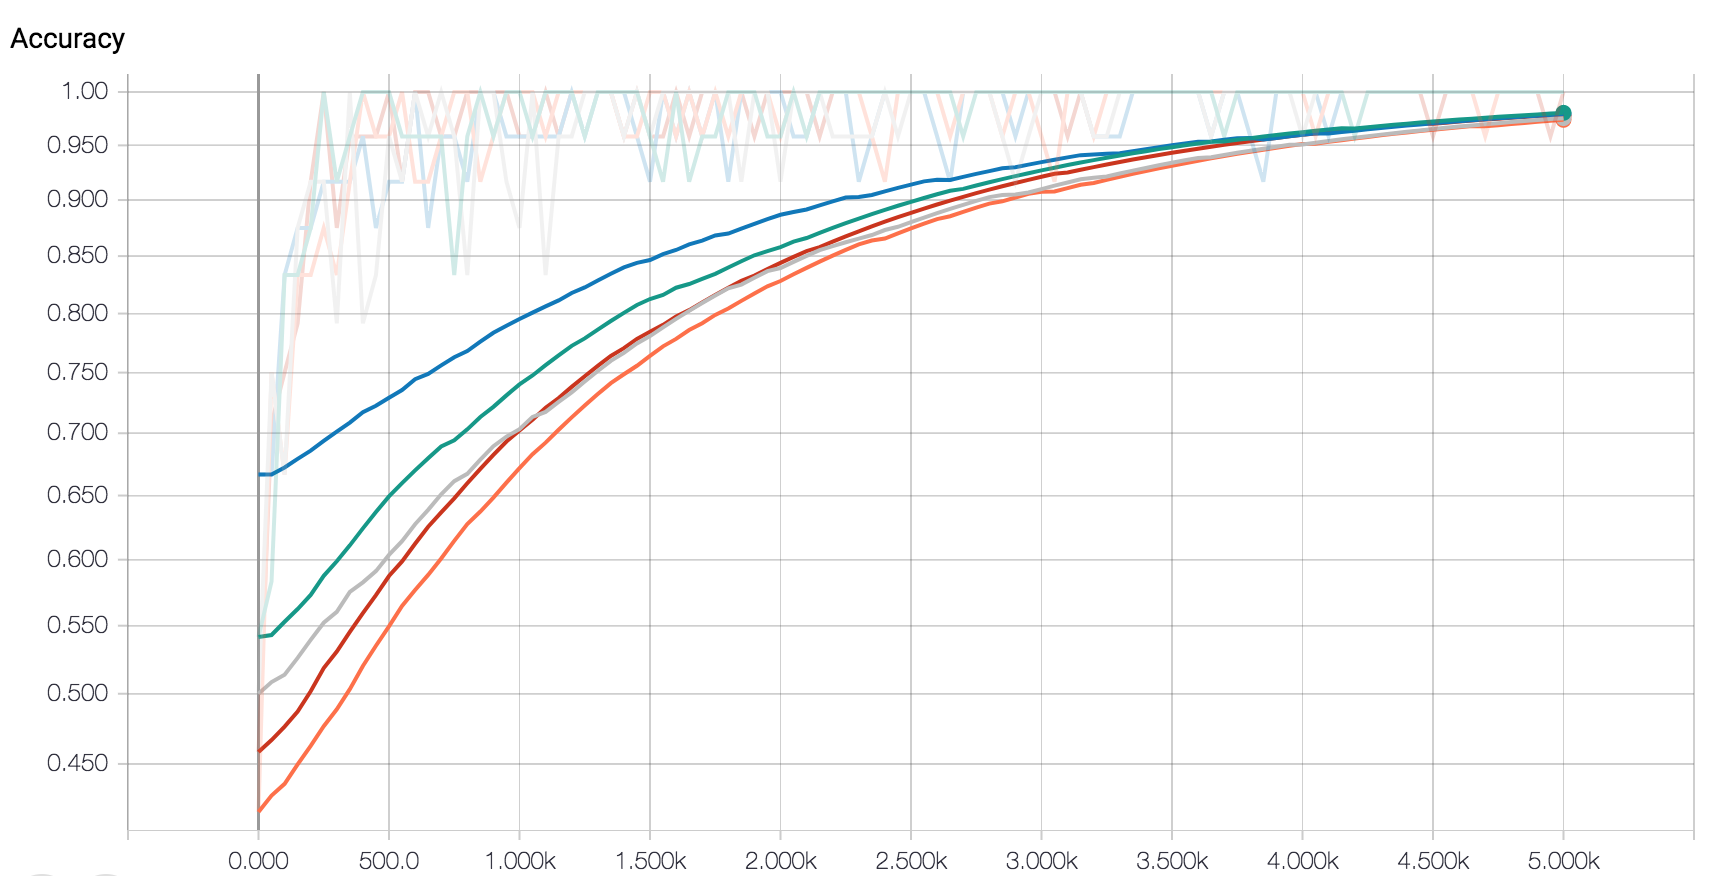
\includegraphics[scale = .24]{acc-unsupervised}
	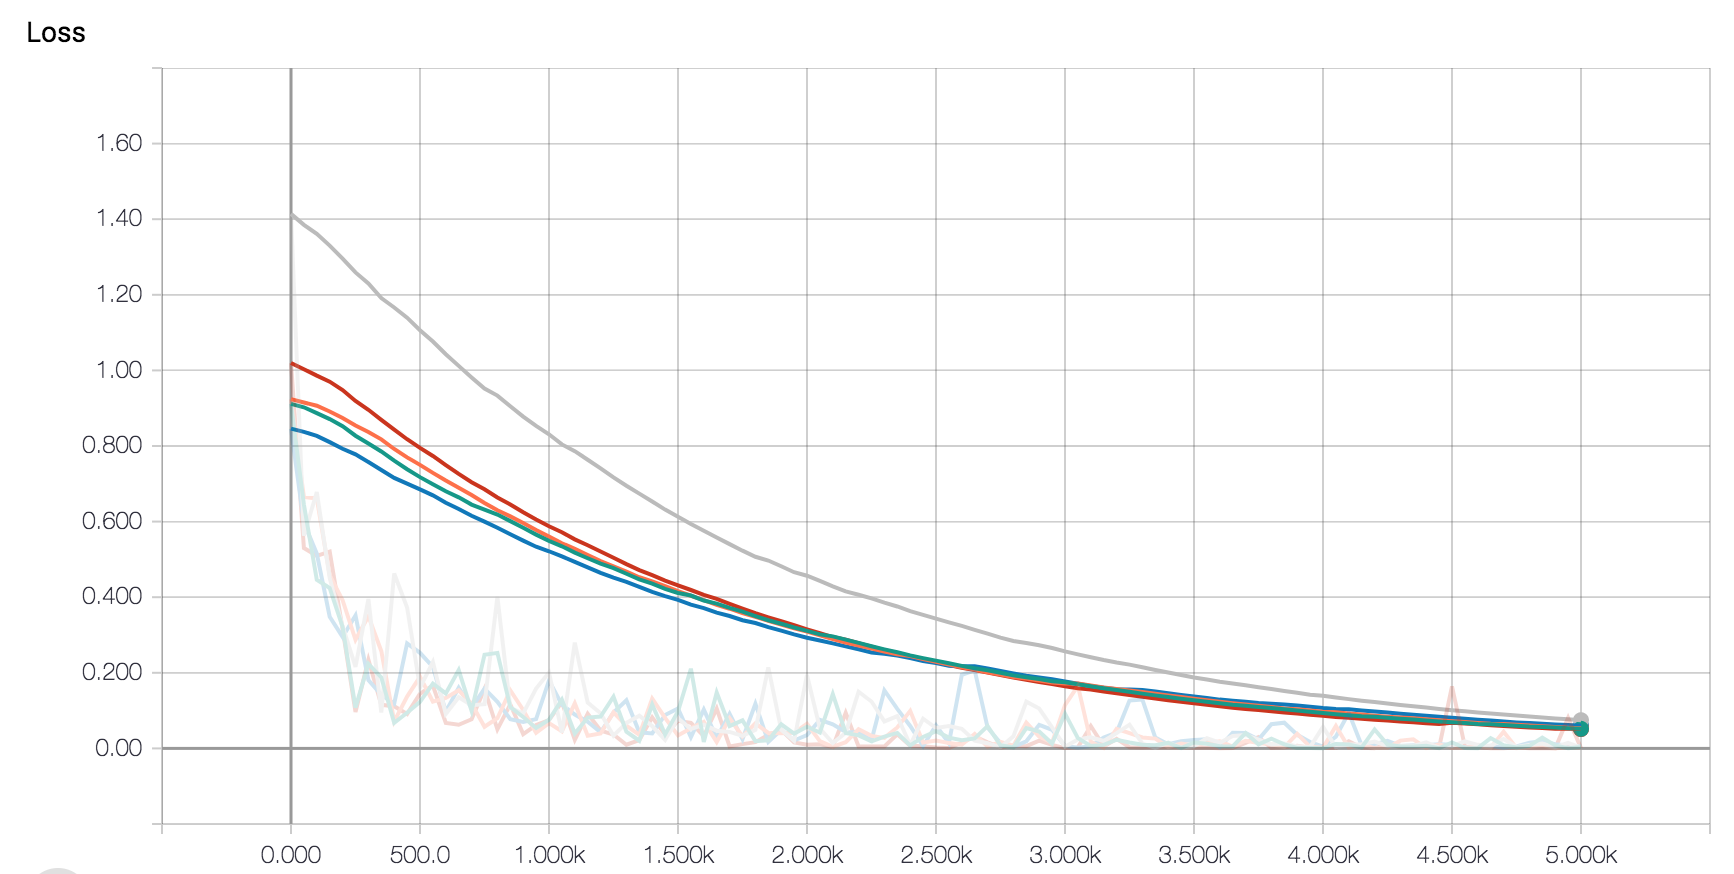
\includegraphics[scale = .24]{unsupervised-success}
	\caption{Training accuracy and loss for each of the five unsupervised iterations over 5000 training iterations each.}
\end{figure}

  \begin{figure}
	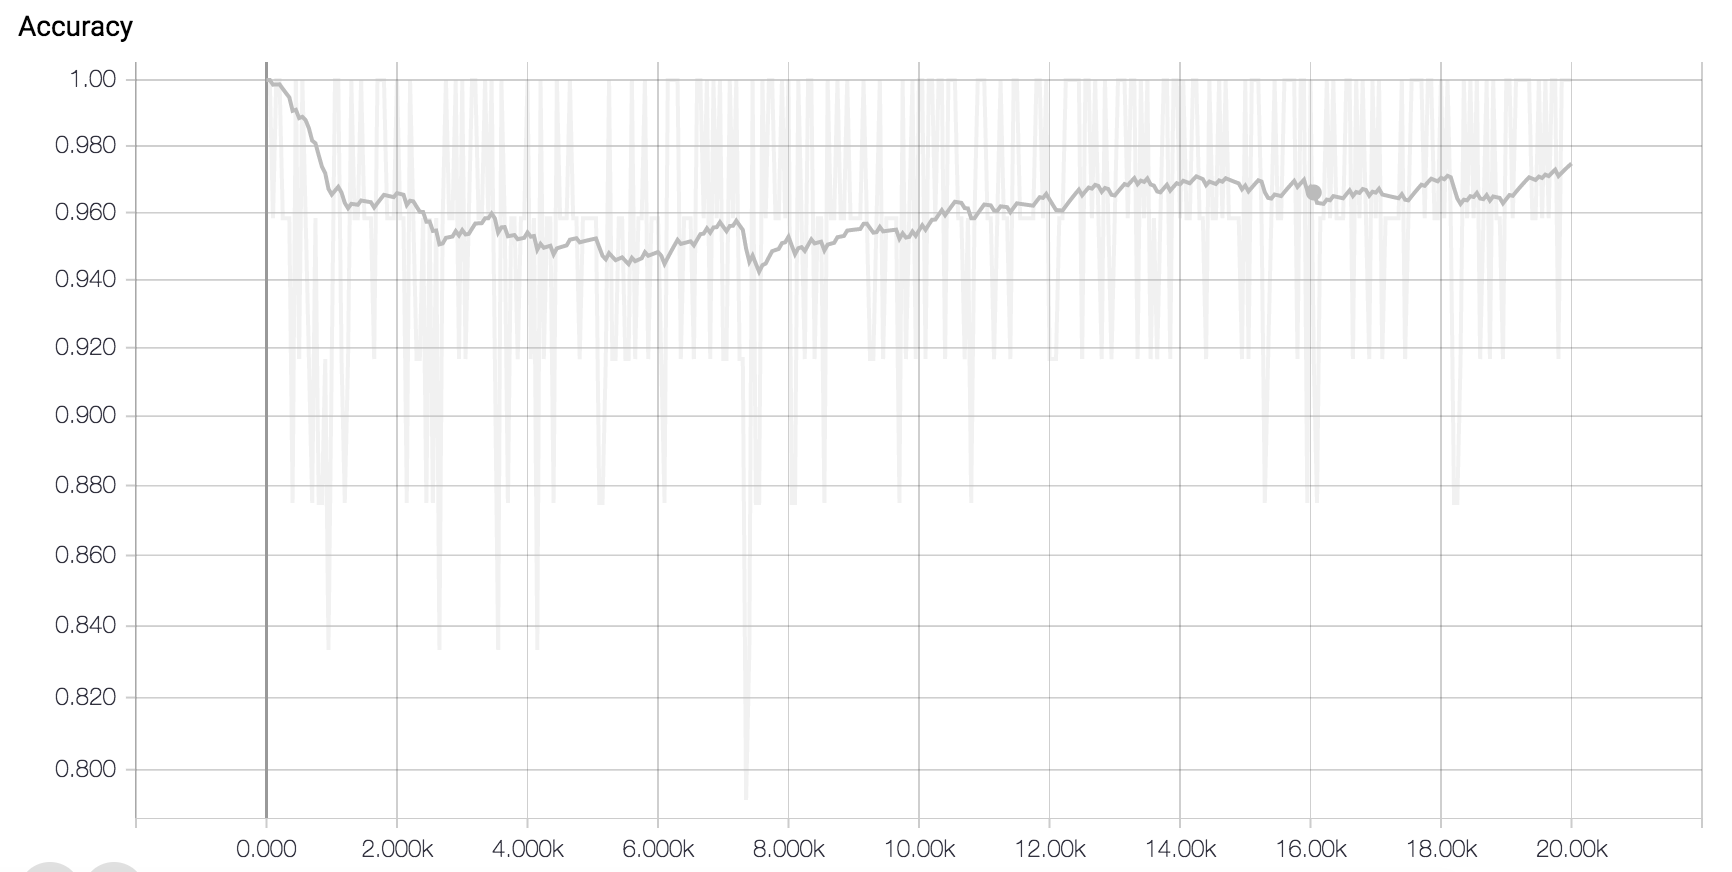
\includegraphics[scale = .24]{unsupervised-failed}
	\caption{Training Accuracy for a single unsupervised iteration of our algorithm on .5 fraction of the data}
\end{figure}


  \begin{figure}
	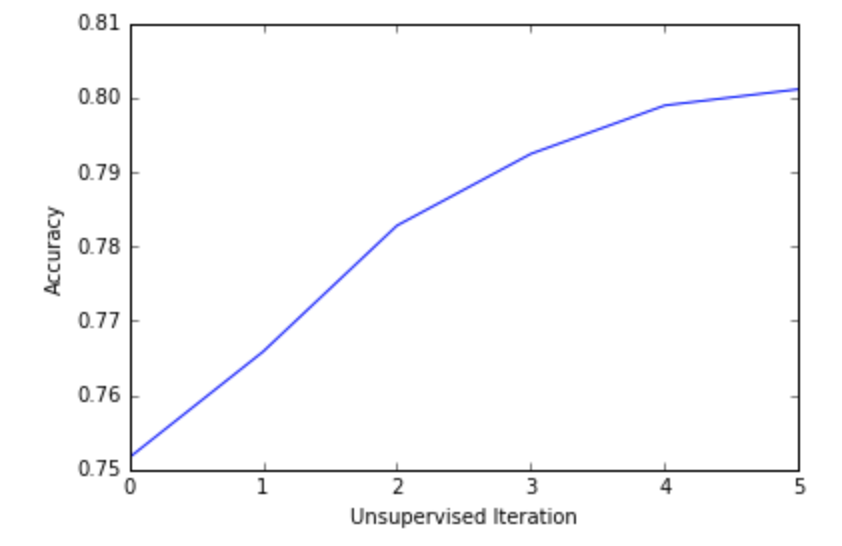
\includegraphics[scale = .5]{unsupervised_iter}
	\caption{Accuracy vs Unsupervised iteration of our algorithm on .1 fraction of the data}
\end{figure}

  \begin{figure}
	\begin{center}
\begin{tabular}{ |c|c| } 
 \hline
 Supervised accuracy (10\% of examples) & 0.7516 \\ 
 Supervised accuracy (10\% labeled, 90\% labeled) & 0.8041 \\ 
 Supervised accuracy (all examples) & 0.8763 \\ 
 \hline
\end{tabular}
\end{center}
	\caption{Final output metrics of supervised and unsupervised learning process on .1 labeled data}
\end{figure}

 
 \clearpage





\section{Conclusions}

We have, in this report, shown the potential feasibility, and also potential downsides of using unsupervised and semi-supervised learning for sequence learning tasks in NLP.

The method we use here might be somewhat effective, but it is in a sense the most "naive" application of unsupervised learning to Sequence learning models. Other work on this topic has also considered other methods (such as rewriting the loss function or using adversial networks) to improve performance on this task. There may be many other improvements that can be made and we may be able to leverage information in unsupervised data even more effectively in the future.

The code for the models and experiments described here can be found at :\begin{verbatim}https://github.com/cynikolai/
Sequence-Cluster-Learner\end{verbatim}

\section{Contributions}










\bibliography{naaclhlt2016}
\bibliographystyle{naaclhlt2016}


\end{document}
